
\documentclass[12pt]{article}

\usepackage{algorithm}
\usepackage{algpseudocode}
\usepackage{enumitem}
\usepackage[body={7in,9.5in},centering]{geometry}
\usepackage{fancyhdr}
\usepackage{times}
\usepackage{tikz}
\usepackage{hyperref}
\usepackage{graphicx}

\lhead{}
\rhead{}
\renewcommand{\headrulewidth}{3pt}
\lfoot{}
\cfoot{}
\rfoot{}
\pagestyle{empty}

\newcommand*\circled[1]{\tikz[baseline=(char.base)]{
            \node[shape=circle,draw,inner sep=2pt] (char) {#1};}}


\begin{document}
\begin{center}
  \Large
  CIS 675 (Fall 2018) Disclosure Sheet 
\end{center} 
\vspace*{2em}

\noindent
\textbf{\Large Name: \underline{ Wentan Bai }} 


\noindent 
\begin{minipage}[t]{1.0\linewidth}

\begin{minipage}[t]{0.25\linewidth}
\textbf{\Large
  HW \# \underline{ 5 }
} 

\end{minipage} \vspace*{3ex}




\begin{minipage}[t]{.8in}
  \textbf{\circled{Yes} \quad No}
\end{minipage}
\qquad 
\begin{minipage}[t]{5.5in}
  Did you consult with anyone on parts of this assignment, including other students, TAs, or the instructor? 
\end{minipage}
\vspace*{1ex}

\begin{minipage}[t]{.8in}
  \textbf{Yes \quad \circled{No}}
\end{minipage}
\qquad 
\begin{minipage}[t]{5.5in}
  Did you consult an outside source (such as an Internet forum or a
  book other than the course textbook) on parts of this assignment? 
\end{minipage}
\vspace*{1ex}

\noindent
  If you answered \textbf{Yes} to one or more questions, please give the details here: \vspace*{5ex} \par
  I also consult all questions and extra question with another student, Wentian Bai. For all questions, we discussed our ideas and I finish my algorithms independently. 


\vfill
\end{minipage}



\vspace*{40ex}

By submitting this sheet through my Blackboard account, I assert that the information on this sheet is true.

%\vfill

\hfill {\tiny This disclosure sheet was based on one originally designed
  by
  Profs. Royer and Older.}


\pagebreak
\noindent
\large Question 1: \vspace{5mm} \par
\normalsize 
Suppose the given grid has $n$ numbers of rows and $m$ numbers of columns. 
\begin{itemize}
  \item On the Westernmost road, all T[i][1] = T[i+1][1] + $d_{i,1}$, 
	since we can only go straight north to the current position at the previous intersection.
  \item	On the Southernmost road, all T[n][j] = T[n][j-1] + $d_{n,j}$,
	since we can only go straight east to the current position at the previous intersection.
  \item Then for remaining intersections, we can go straight east or straigth north to the current position at the previous intersections.
	Therefore, we choose the shorter one, T[i][j] = $d_{i,j}$ + \textbf{min}(T[i+1][j], T[i][j-1])
\end{itemize}

\begin{algorithm}
\begin{algorithmic}
\State T[n][m]
\State T[n][1] = $d_{n,1}$
\State \textbf{For} i $\leftarrow$ n-1 to 1 \textbf{:}
\State \hspace{0.4cm} T[i][1] $\leftarrow$ T[i+1][1] + $d_{i,1}$
\State \textbf{For} j $\leftarrow$ 2 to m \textbf{:}
\State \hspace{0.4cm} T[n][j] $\leftarrow$ T[n][j-1] + $d_{n,j}$
\\
\State \textbf{For} i $\leftarrow$ n-1 to 1 \textbf{:}
\State \hspace{0.4cm} \textbf{For} j $\leftarrow$ 2 to m \textbf{:}
\State \hspace{0.8cm} T[i][j] = $d_{i,j}$ + \textbf{min}(T[i+1][j], T[i][j-1])
\\
\State \textbf{Return} T[1][m] 
\end{algorithmic}
\end{algorithm}
\noindent \\
\textbf{running time:} \par
We iterate through all intersections so the final time is $O(n^2)$.



\pagebreak
\noindent
\large Question 2: \vspace{5mm} \par
\normalsize 
This question is similar as Splitting a String.
I need to write a helper function to determine whether a particular string is a palindrome.

\begin{itemize}
  \item we check if a sub string from i to j is a palindrome. 
	If current sub string is a palidrome, we check if the previous sub string is a palidrome, which result is saved at Seq(i-j-1).
	If all requirements are satisified, save Seq(i) as True.
  \item The helper function is to determine whether a particular string is a palindrome. 
	We iterate from head and tail to center at the same time. 
	If there are a pair of characters which are different, this particular string is not a palindrome.
\end{itemize}

\begin{algorithm}
\begin{algorithmic}
\State Seq(i) = False
\State Seq(0) = True
\State \textbf{For} i = 1 to n \textbf{:}
\State \hspace{0.4cm} \textbf{For} j = 1 to i \textbf{:}
\State \hspace{0.8cm} \textbf{if} \textbf{helper}(Seq[i-j ... i]) == True and Seq(i-j-1) == True
\State \hspace{1.2cm} Seq(i) $\leftarrow$ True
\State \textbf{Return} Seq(n)
\end{algorithmic}
\end{algorithm}
Following is helper function: 
\begin{algorithm}
\begin{algorithmic}
\State def \textbf{helper}(Seq)
\State \hspace{0.4cm} \textbf{if} length(Seq) == 1 or 0
\State \hspace{0.8cm} \textbf{Return} False
\State \hspace{0.4cm} i = 0, j = length(Seq) - 1
\State \hspace{0.4cm} \textbf{While} i $\not=$ j and i $<$ j \textbf{:} 
\State \hspace{0.8cm} \textbf{if} Seq[i] $\not=$ Seq[j] \textbf{:}
\State \hspace{1.2cm} \textbf{Return} False
\State \hspace{0.8cm} i++, j- -
\State \hspace{0.4cm} \textbf{Return} True
\end{algorithmic}
\end{algorithm}
\noindent \\
\textbf{running time:} \par 
When we iterate through all sub strings, and each helper function need $O(n)$ time so finally we need $O(n^3)$.
The final time is $O(n^2)$


\pagebreak
\noindent
\large Question 3: \vspace{5mm} \par
\normalsize 
By hint, I modify the graph. 
In original graph, there are not capacities on the edges, so I will add capacities for each edges.

\begin{itemize}
  \item Assign $\infty$ or the sum of capacities of all nodes to the capacities of all edges leaving from source node. 
  \item If the current node is only pointed by one node and only one edge leaves from this node.
	Then assign the same size of capacity on current node to the edge leaving from current node. 
  \item If the current node $u$ points to multiple nodes or is pointed by multiple nodes, 
	then make node $u$ only connect with a new node $v$ which has the same capacity.
	Then assign the same size of capacity on node $u$ to the $Edge(u, v)$ 
	Connect node $v$ to the nodes which are original pointed by node $u$. 
	Assign the same size of capacity on node $u$ to the capacities of these new edges.  	

\end{itemize}
\par
Following is an example. The first one is original graph and the second is modified graph. \\
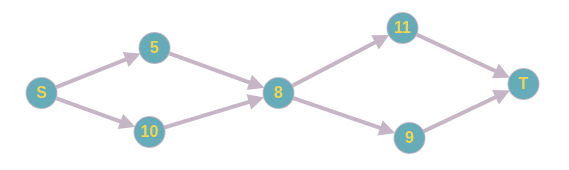
\includegraphics[width=12cm, height=4cm]{question3L} \\
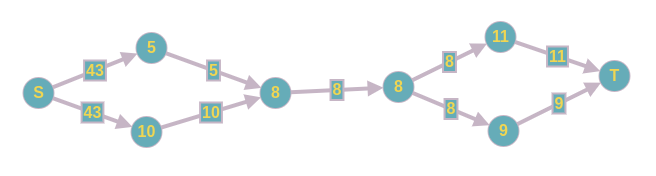
\includegraphics[width=15cm, height=4cm]{question3R} 

\par
We can find a max flow using original maximum flow algorithm on the modified graph.
\\

\textbf{running time:} \par
The time is the same as the time of original maximum flow algorithm, $O(|V|\cdot|E|^2)$.



\pagebreak
\noindent
\large Question 4: \par
\normalsize 
My algorithm is: 

\begin{itemize}
  \item Create a node for each animal denoted as $a_i$. Then create a node for each doctor denoted as $D_j$. Create a source node $s$ and a sink node $t$. 
  \item Draw edges from source node to every node $a_i$, and each $Edge(s, a_i)$ has a capacity $h_i$.
	Input flow is the time of the animals to be treated.
  \item If animal $a_i$ can be treated by doctor $D_j$, draw a edge from $a_i$ to $D_j$, and each $Edge(a_i, D_j)$ has a capacity $C_j$.
  \item Draw edges from every doctor $D_j$ to sink node $t$, and each $Edge(D_j, t)$ has a capacity $C_j$. 
	This setp ensures each doctor $j$ works at most $C_j$ time. 
  \item Run maximum flow algorithm on this graph. 
	Look at which edges between aminal nodes and doctor nodes has flow along with them; 
	these edges correspond to the assignment animals to dockers.

\end{itemize}

Following is an example. \\
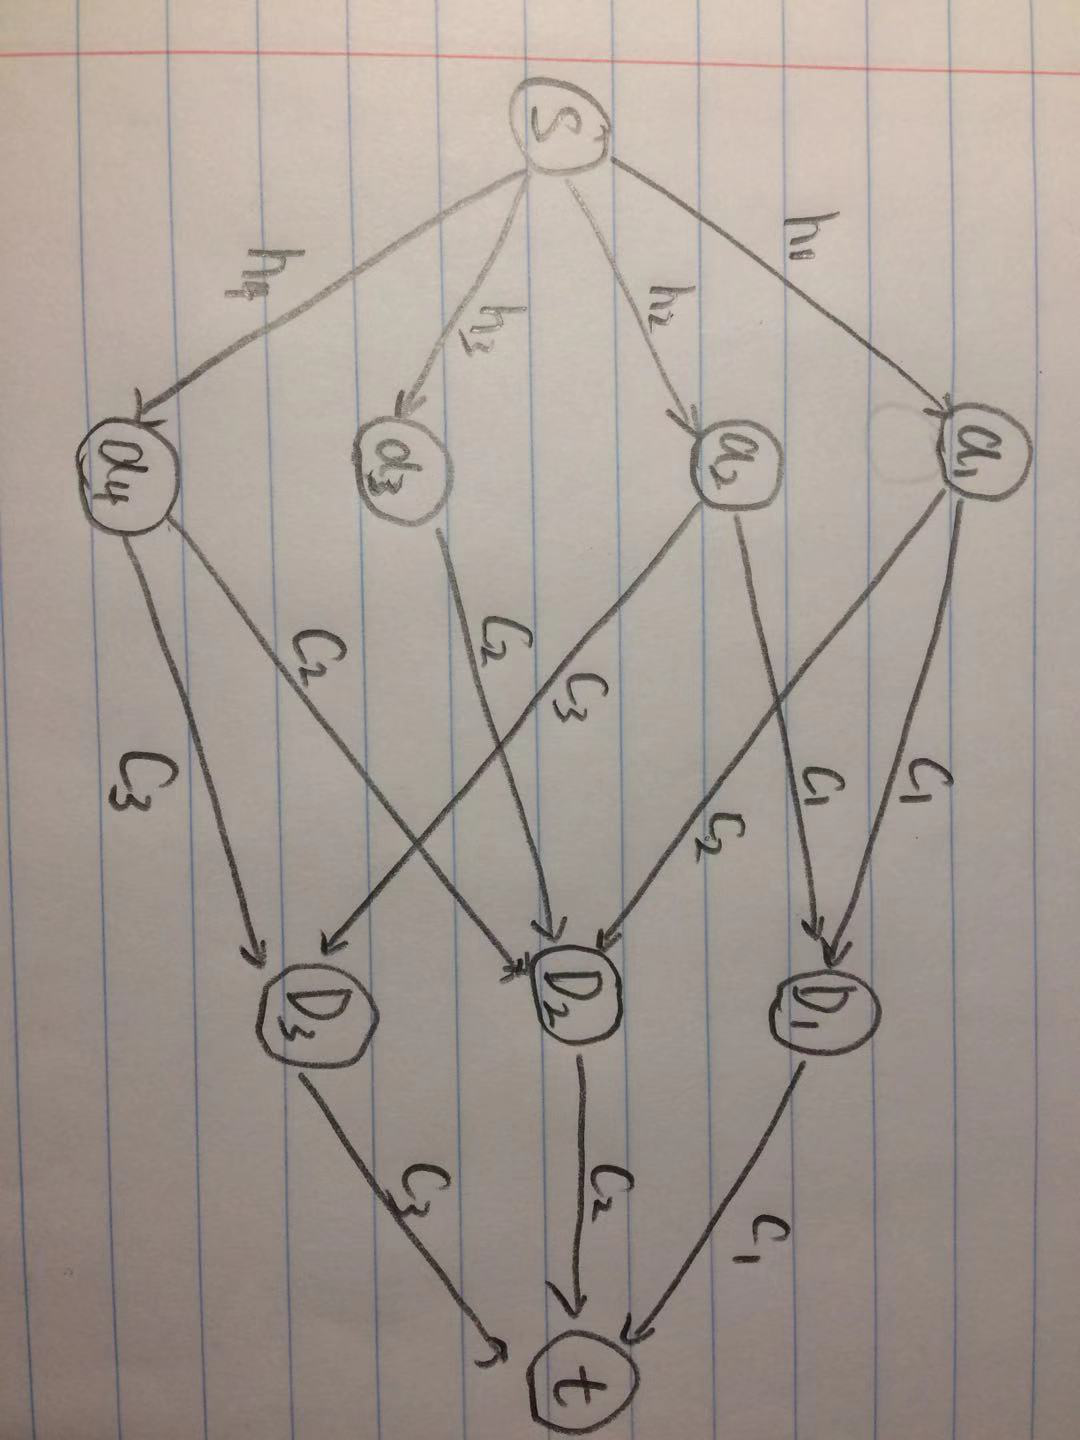
\includegraphics[width=6cm, height=10cm, angle=90,origin=c]{question4}
\par
We can get the answer by using original maximum flow algorithm on this graph.
\\

\textbf{running time:} \par
The time is the same as the time of original maximum flow algorithm, $O(|V|\cdot|E|^2)$.




\pagebreak
\noindent
\large Question 5: \par
\normalsize 
My algorithm is:
\begin{itemize}
  \item	Create a node for each paper denoted as $p_j$, and create a node for each reviewer denoted as $R_i$. Create a source node $s$ and a sink node $t$.
  \item Draw edges from source node to every node $p_j$, and each $Edge(s, p_j)$ has a capacity $3$. 
  \item Draw a edge from each node $p_j$ to every node $R_i$ if paper $p_j$ is not submitted by reviewer $R_i$.  
	Each $Edge(p_j, R_i)$ has a capcity 1. 
  \item Draw edges from every node $R_i$ to sink node, and each $Edge(s, p_i)$ has a capacity $m_i$.
  \item Run maximum flow algorithm. 
	Look at which edges between paper nodes and reviewer nodes has unit 1 of flow along with them; 
	these edges correspond to the assignment papers to reviewers.
	In this algorithm, we must ensure that each node $p_j$ is reviewed by 3 times. 
	So the final flow into sink node should be 3 times of numbers of papers.
\end{itemize}

\noindent \\
\textbf{running time:} \par
The time is the same as the time of original maximum flow algorithm algorithm, $O(|N + M|\cdot|N + M|^2) = O(|N + M|^3)$.



\pagebreak
\large \textbf{Extra}:\\ \vspace{5mm}\par
\normalsize 
Create an array $dp[M][N]$: $dp[i][j]$ presents we need to choose $i$ numbers of fruits from $j$ numbers of boxes. \par
In initialization, if $m_1$ $\geq$ 1, assign $dp[1][1]$ to 1; else assign $dp[1][1]$ to 0. \par
For all $dp[1][2]$ to $dp[1][N]$, in each step $j$, if $m_j$ $\geq$ 1, then assign $dp[1][j]$ = $dp[1][j - 1] + 1$; else assign $dp[1][j] = dp[1][j - 1]$. 
In each step $j$, we need to choose one fruit from $j$ numbers of boxes. 
If $B_j$ is not empty, then there will be $dp[1][j - 1] + 1$ ways to choose.
Otherwise, there are still the $dp[1][j - 1]$ numbers of ways. \par
For all $dp[2][1]$ to $dp[M][1]$, in each step $i$, if $m_1$ $\geq$ $i$, then assign $dp[i][1] = 1$; else assign $dp[i][1] = 0$. 
In each step $i$, we need to choose $i$ numbers of fuits from $B_1$.
If $m_1$ is larger than required numbers of fruits $i$, then there is one type to choose; 
Otherwise, there is not enough numbers of fruits to choose. \par
Iterate from $i = 2$ to $M$, and for each i, iterate from $j = 2$ to $N$, 
and in each step $i$ $j$, assign $dp[i][j] = dp[i - 1][j] + dp[i][j - 1]$. \par
The final result is in $dp[M][N]$.


\begin{algorithm}
\begin{algorithmic}
\State dp[M][N]
\State dp[1][1] $\leftarrow$ 0
\\
\State \textbf{For} j = 2 to N :
\State \hspace{0.4cm} \textbf{If} $m_j$ $\geq$ 1 \textbf{:}
\State \hspace{0.8cm} $dp[1][j]$ $\leftarrow$ $dp[1][j - 1] + 1$
\State \hspace{0.4cm} \textbf{Else :}
\State \hspace{0.8cm} $dp[1][j]$ $\leftarrow$ $dp[1][j - 1]$
\\
\State \textbf{For} i = 2 to M :
\State \hspace{0.4cm} \textbf{If} $m_1$ $\geq$ $i$ \textbf{:}
\State \hspace{0.8cm} $dp[i][1]$ $\leftarrow$ 1
\State \hspace{0.4cm} \textbf{Else :}
\State \hspace{0.8cm} $dp[i][1]$ $\leftarrow$ 0
\\
\State \textbf{For} i = 2 to M :
\State \hspace{0.4cm} \textbf{For} j = 2 to N :
\State \hspace{0.8cm} $dp[i][j]$ $\leftarrow$ $dp[i - 1][j] + dp[i][j - 1]$
\\
\State \textbf{return} $dp[M][N]$
\end{algorithmic}
\end{algorithm}


\textbf{running time:} \par
Interation from 2 to M using M time, and for each step, interation from 2 to N using N time.
Therefore, the final time is $O(N M)$


\end{document} 







